% Chapter Template

\chapter{Evaluation} % Main chapter title

\label{Chapter7} % Change X to a consecutive number; for referencing this chapter elsewhere, use \ref{ChapterX}

TODO review the core goals outlined in the introduction, and
methodically review how well my final prototypes stack up against those
goals. This section serves to prove (with all the data) that the
approach I've described in the previous chapters actually works.

TODO a huge portion of this chapter can come from the "Interesting
Graphs for my Thesis" document.

\section{Benchmarks}
\label{sec:evaluation-benchmarks}

This chapter will use four key benchmarks to assess the effectiveness
of the design proposed in Chapters \ref{Chapter4}, \ref{Chapter5}, and
\ref{Chapter6}. These metrics are:

\begin{itemize}

    \item \emph{Compatibility with Standard Speedcubes}: How
    effectively can the design be deployed in a standard, non-smart
    speedcube without any permanent modifications or reducing the
    cube's performance? (Section
    \ref{sec:compatibility-with-standard-speedcubes})
    
    \item \emph{Move Tracking Accuracy}: How accurately can the design
    track the moves performed on the modified speedcube? (Section
    \ref{sec:move-tracking-accuracy})
    
    \item \emph{Move Tracking Granularity}: What other metrics can the
    each face turn. (Section \ref{sec:move-tracking-granularity})
    design provide? Of greatest interest is the time spent executing
    
    \item \emph{Competition Legality}: To what extent is the design
    compliant with existing competition regulations? (Section
    \ref{sec:competition-legality})
    
\end{itemize}

Each of these metrics will be discussed and analyzed in detail in the
following sections.

\section{Compatibility with Standard Speedcubes}
\label{sec:compatibility-with-standard-speedcubes}

Since a major goal of this research project is to allow speedcubers to
practice with the same cube they compete with, it is imperative that
the proposed design function without requiring permanent modifications
to the original speedcube. For the same reason, the design must also
retain the original performance of the speedcube as much as possible.

As shown in Figure \ref{fig:core-placement}, the proposed PCB
transmitter can be deployed in a Gans 356 speedcube by simply changing
out the original centercap for a custom-built one containing the
transmitter. The modifications to the cube are purely temporary since
the original cube can be perfectly restored by simply replacing the
original centercaps.

The performance impact of the custom centercaps with the transmitters
is also small since the little weight they add to the cube is placed
close to the axes of rotation. On the Gans 356, a stock centercap has a
mass of 0.6719 grams, while the custom centercap shown in Figure
\ref{sec:miniaturization} has a mass of 1.6905 grams. Multiplying the
approximately 1.2 gram difference per centercap by the six centercaps
on the cube results in a 7.2 gram increase in mass for the entire
speedcube. Since the stock Gans 356 has a mass of 84.1204 grams, this
is only an 8.6\% increase in mass, which is within the range of
variation between different speedcubes. This additional weight does
increase the moment of interia of each face; however, this increase is
small because the added weight placed close to the axes of rotation. As
such, the corresponding performance penalty of the extra weight would
be small.


\section{Move Tracking Accuracy}
\label{sec:move-tracking-accuracy}

For the design to be usable it must be able to track the moves of a
traditional, non-smart speedcube. Furthermore, since untracked moves
render the final move sequence invalid unless manually reviewed and
corrected, it is critical that the design detect moves with high or
perfect accuracy.

This particular benchmark was measured by running the receiver detailed
in Chapter \ref{Chapter5} through a battery of tests. These tests
consisted of running several noisy synthetic audio sequences (see
Section \ref{sec:adding-realistic-noise}) through the receiver algorithm
with a variety of parameters and comparing the detected move sequence
to the one used to generate the audio.

The specific move sequence used for the analysis was the "demo alg"
shown in Figure \ref{fig:example-alg-audio} because it sweeps through
every possible centerpiece state. The synthetic audio for this move
sequence was generated at 2 TPS and 5 TPS, then augmented with the
background noise of three different speedcubes (the Gans 356, Gans X,
and QiYi QiMeng) for a total of 6 audio samples. Each of these six
audio samples was run through the receiver algorithm for each of the
720 possible combinations of 10 window sizes, 12 standard deviation
multipliers, and 6 minimum thresholds. The resulting detected move
sequence from each run was then compared with the original "demo alg"
to determine a percent similarity as a measure of the accuracy of the
receiver under each set of parameters.

\newpage
\subsection{Number of Perfect Detections}
\begin{figure}
\begin{subfigure}{\textwidth}
    \centering
    \caption{Total number of perfect detections by cube}
    \label{fig:perfect-detections-by-cube}
    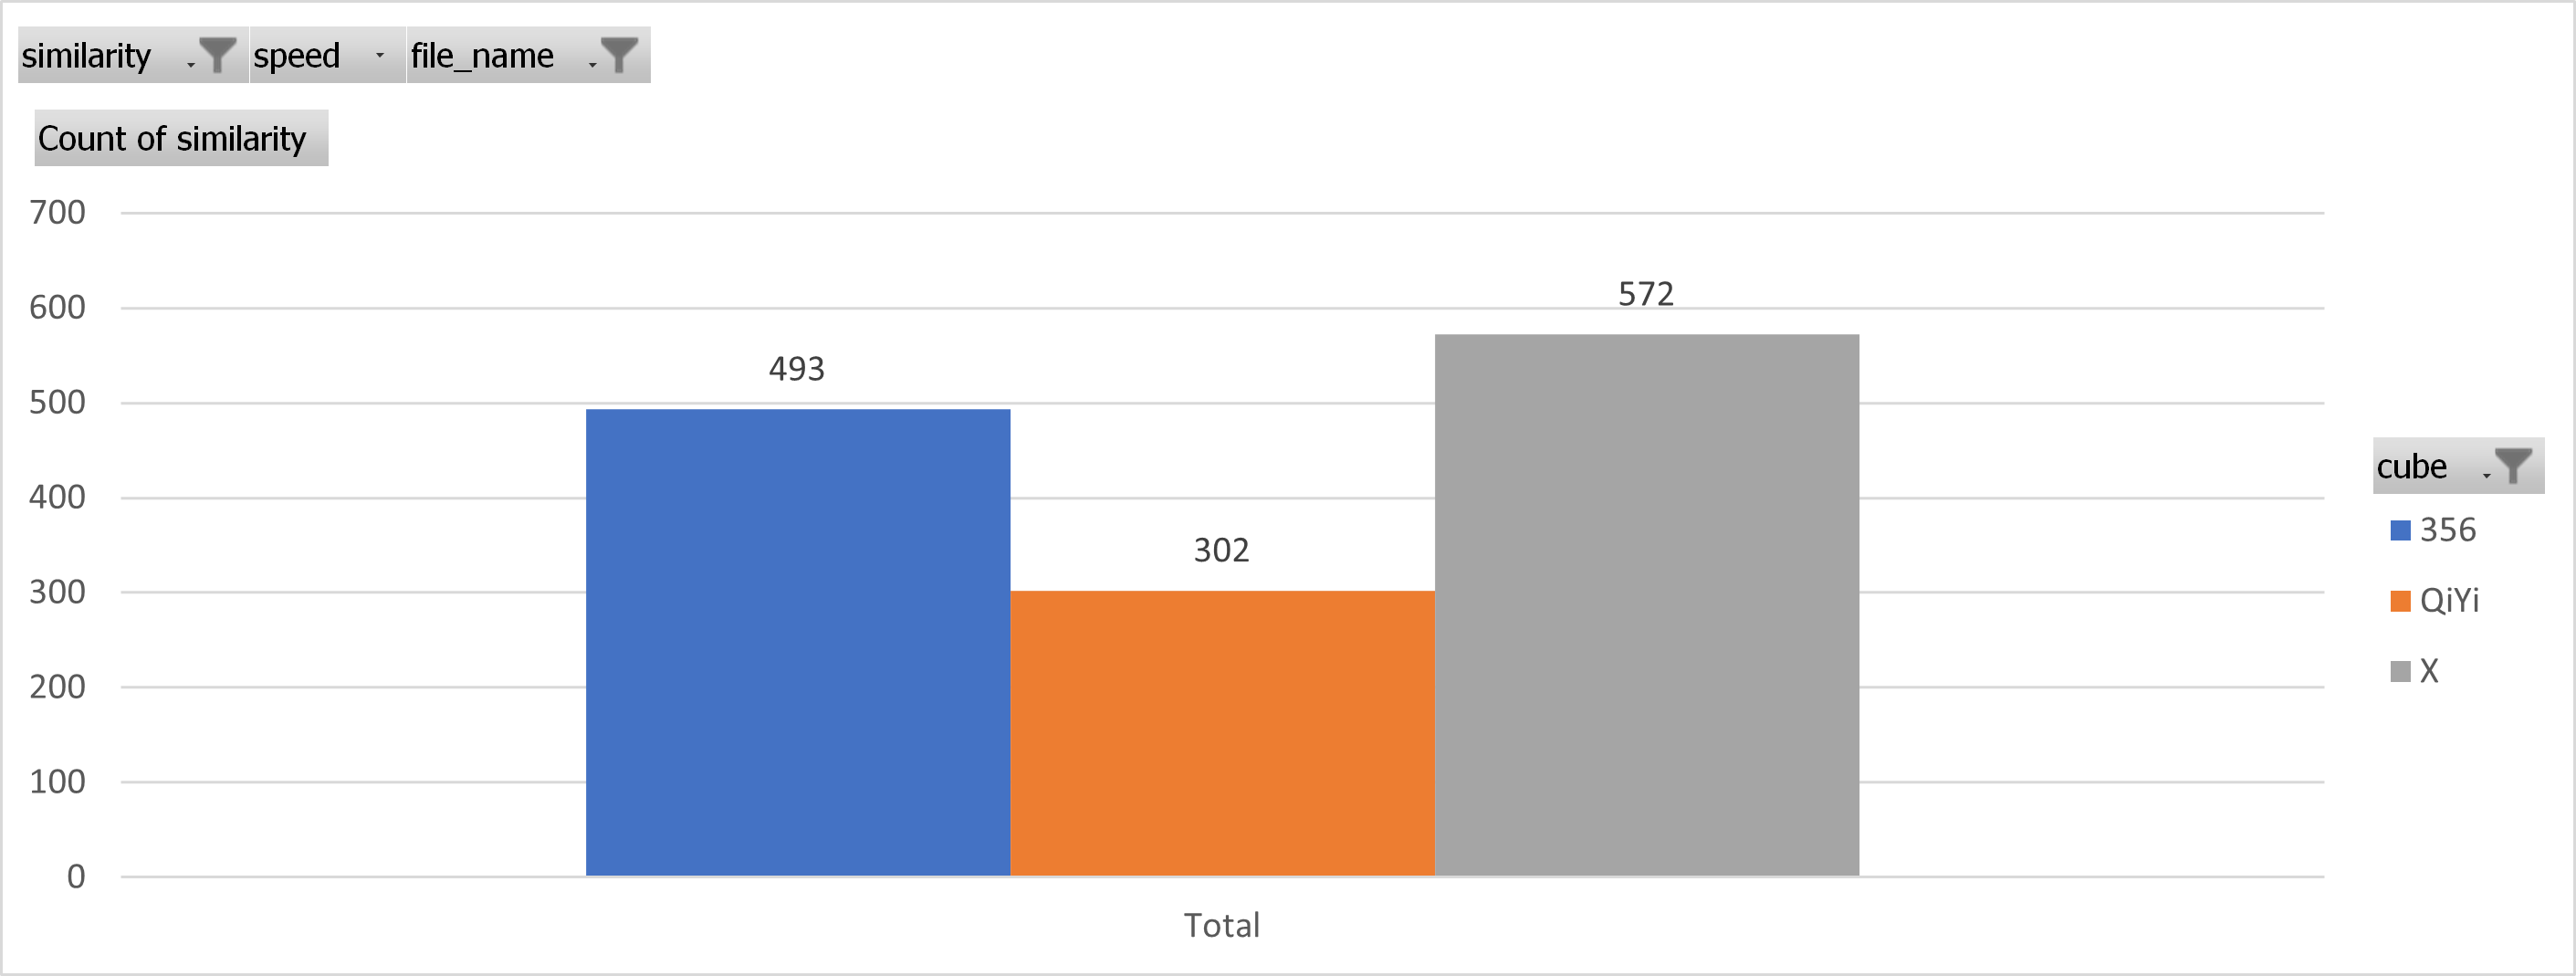
\includegraphics[width=0.75\linewidth]{Figures/7 Evaluation/perfect_detections_by_cube.png}
\end{subfigure}\\

\begin{subfigure}{\textwidth}
    \centering
    \caption{Total number of perfect detections by window\_size}
    \label{fig:perfect-detections-by-window-size}
    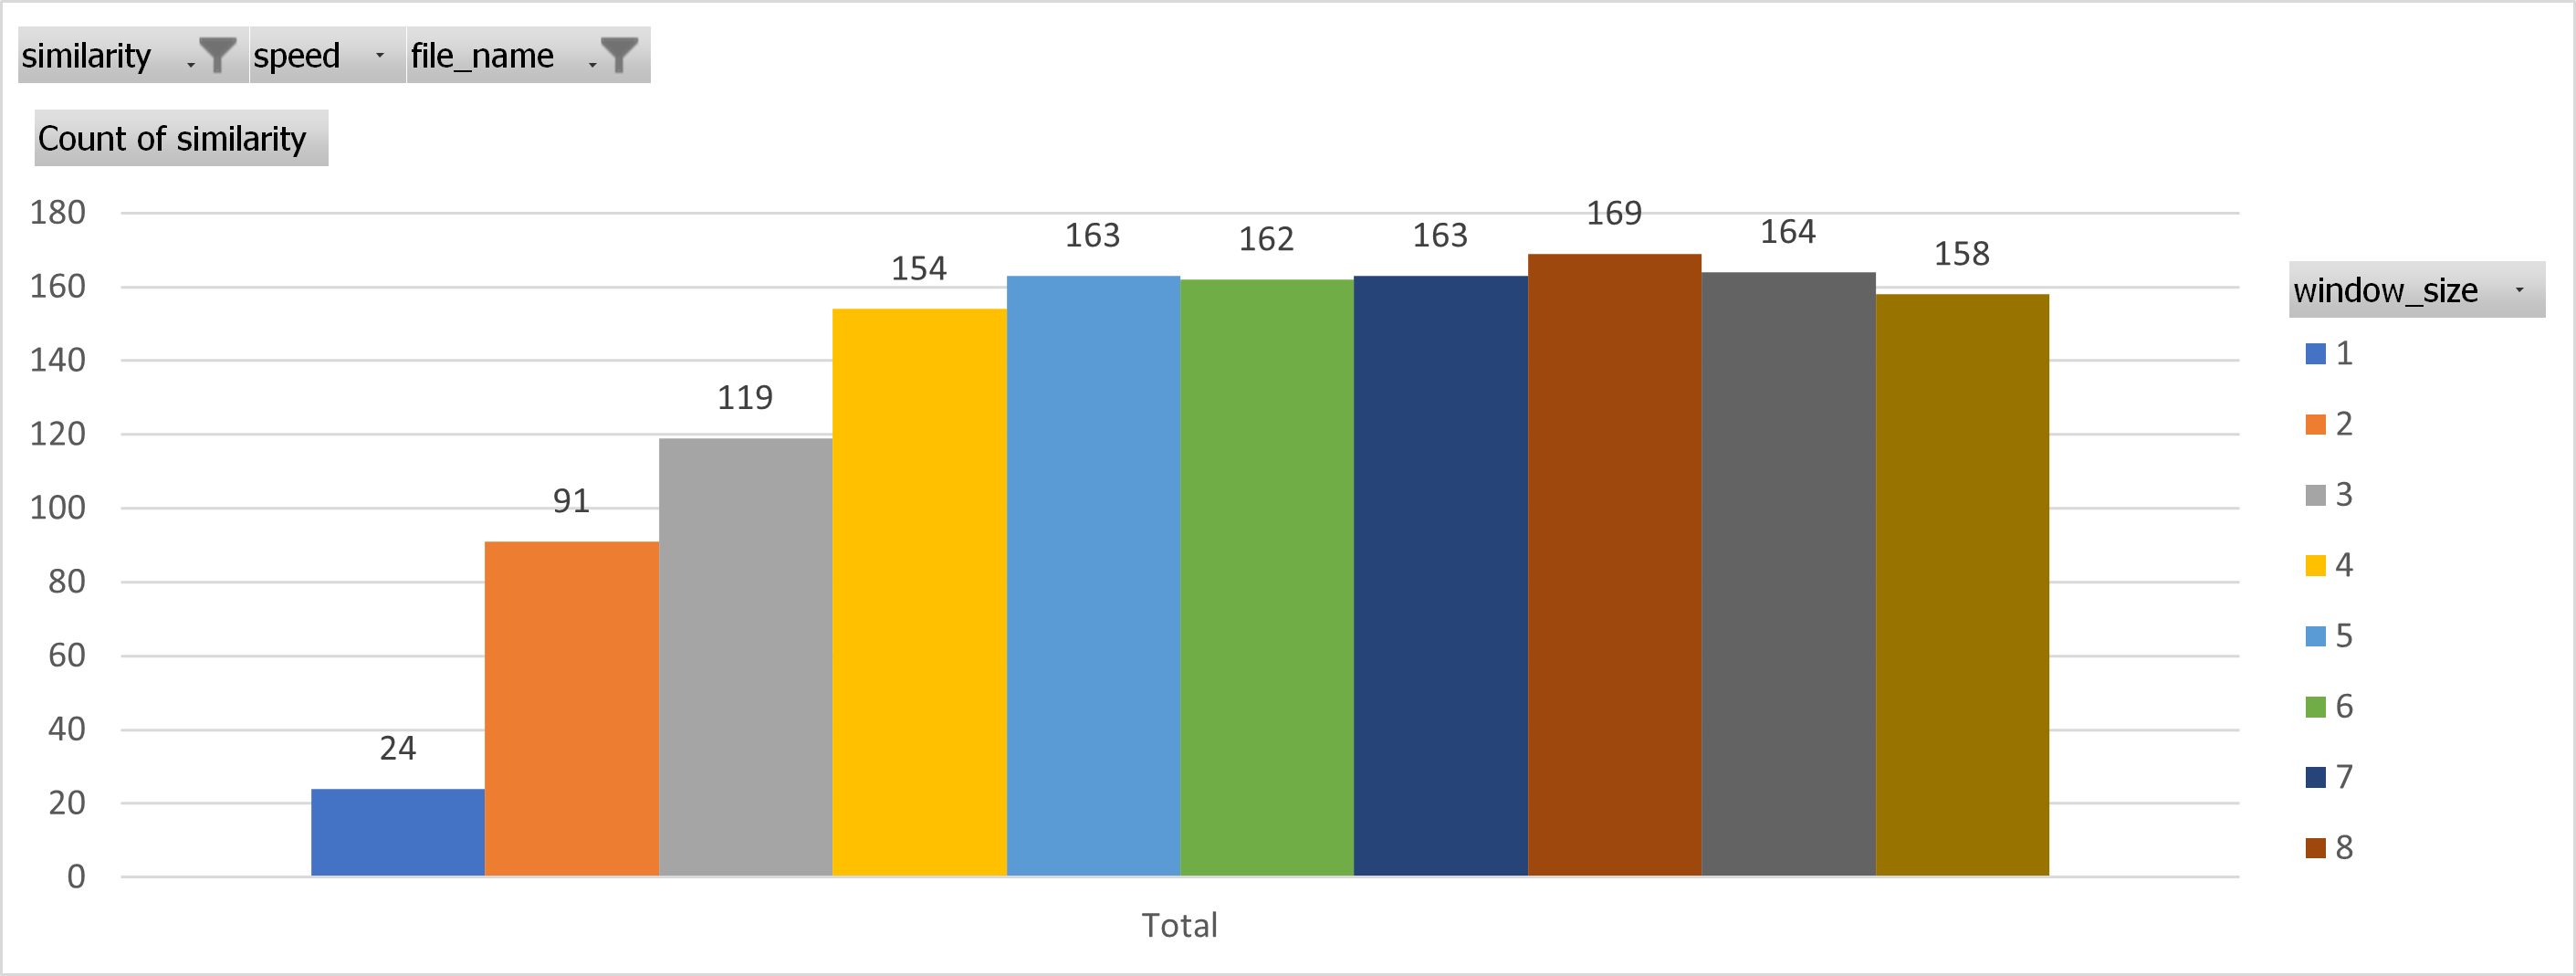
\includegraphics[width=0.75\linewidth]{Figures/7 Evaluation/perfect_detections_by_window_size.png}
\end{subfigure}\\

\begin{subfigure}{\textwidth}
    \centering
    \caption{Total number of perfect detections by stdv multiplier}
    \label{fig:perfect-detections-by-stdv}
    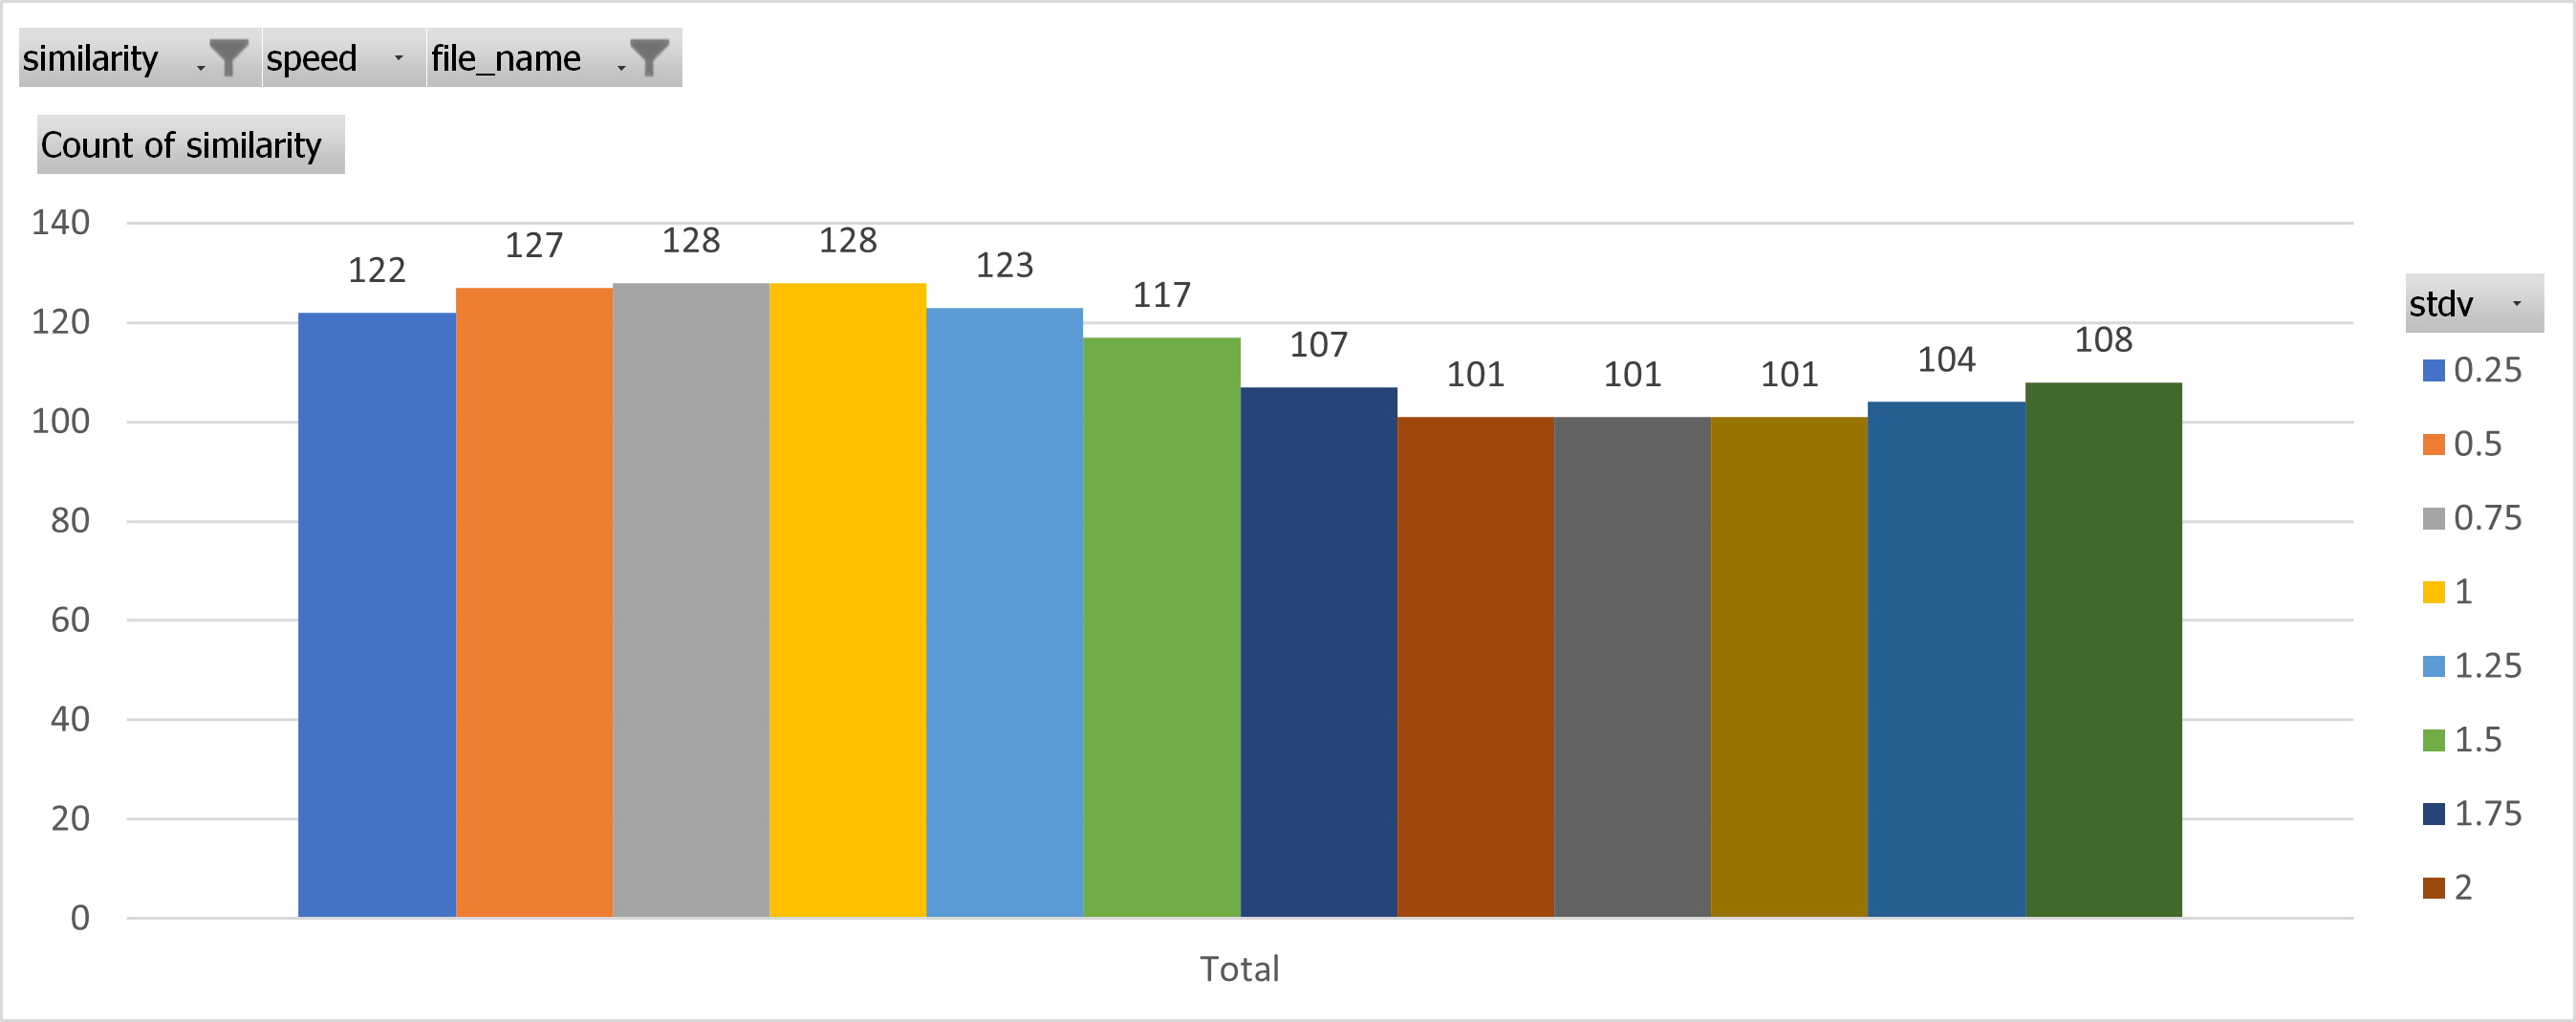
\includegraphics[width=0.75\linewidth]{Figures/7 Evaluation/perfect_detections_by_stdv.png}
\end{subfigure}\\

\begin{subfigure}{\textwidth}
    \centering
    \caption{Total number of perfect detections by alt\_min}
    \label{fig:perfect-detections-by-alt-min}
    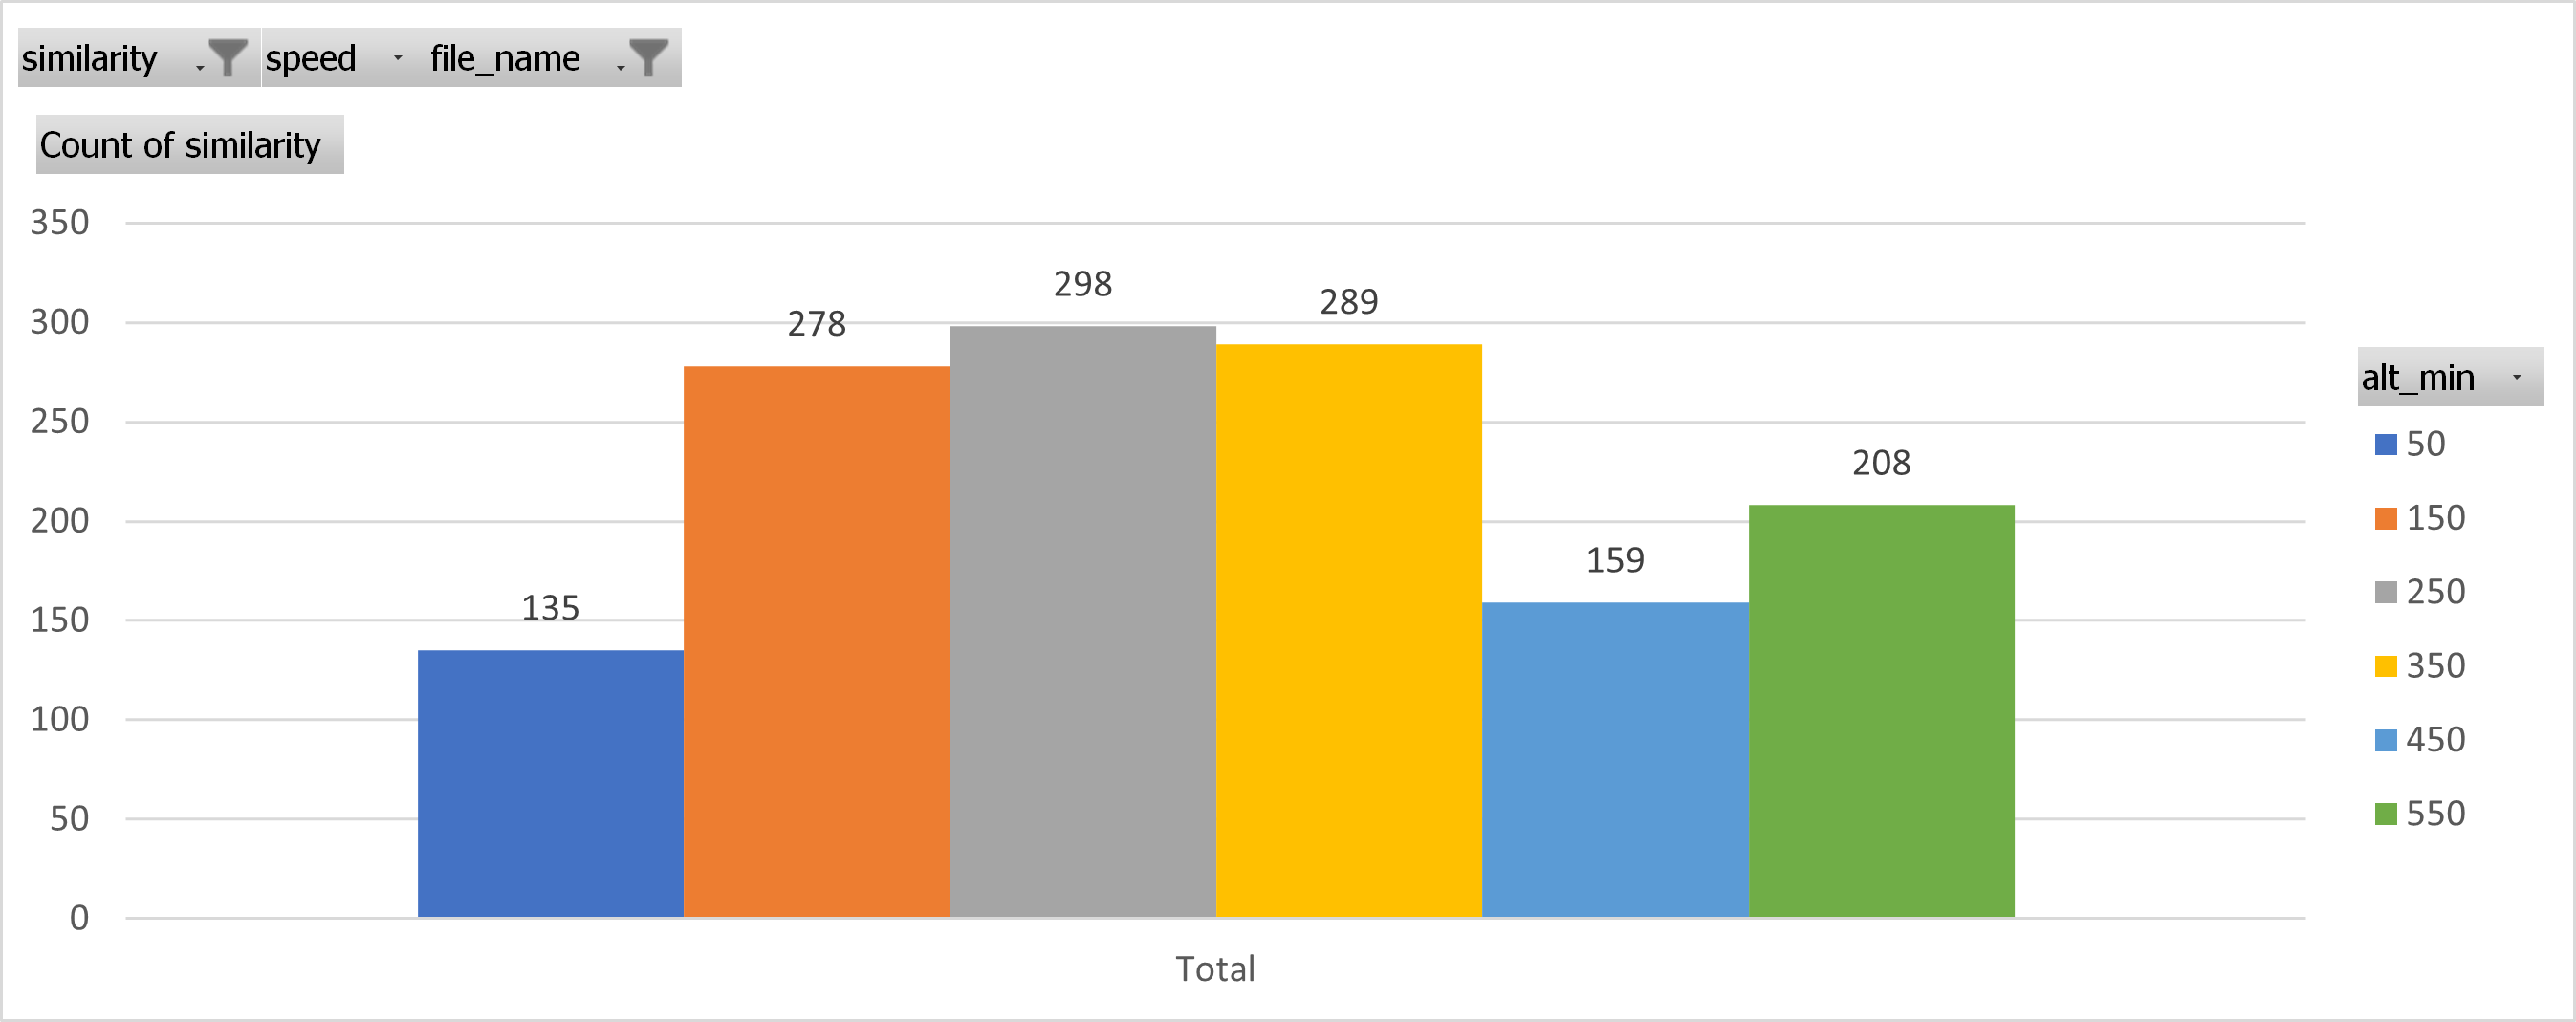
\includegraphics[width=0.75\linewidth]{Figures/7 Evaluation/perfect_detections_by_alt_min.png}
\end{subfigure}\\
\end{figure}

\subsection{Influence of Standard Deviation Multiplier}

\begin{figure}[h]
    \centering
    \caption{Effect of stdv multiplier on accuracy of detection by cube}
    \label{fig:similarity-by-cube}
    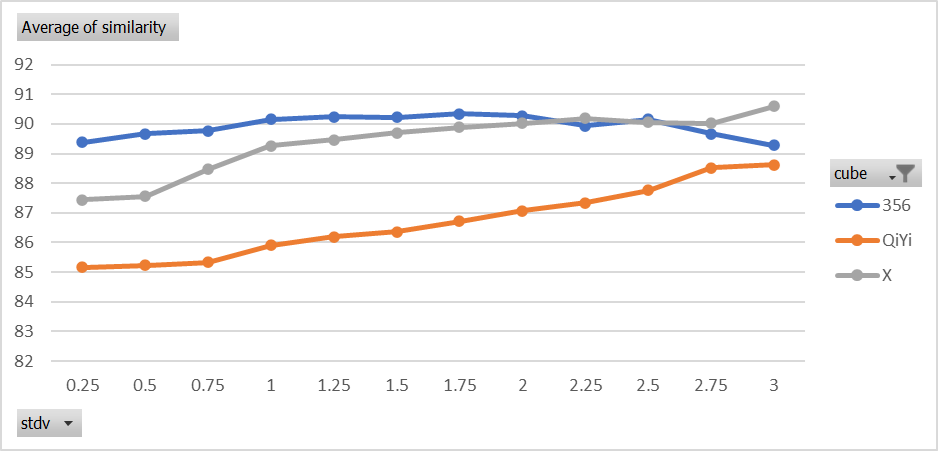
\includegraphics[width=0.75\linewidth]{Figures/7 Evaluation/similarity_by_cube.png}
\end{figure}

The 356 is the quietest cube which means its use does not add much
noise to the signal. As a result, it is not surprising that it performs
well with a low stdv multiplier. What is surprising is the degradation
of accuracy after reaching a multiplier of 2.

The QiYi is the noisiest of the three which explains its poor
performance with low multipliers. It is interesting that its accuracy
rises consistently with an increase in the stdv multiplier, although we
can see a slight taper in the rate of increase in the shift from 2.75
to 3. It would also be interesting to see how the QiYi performs at
higher multipliers (e.g. 4, 5 or higher).

The X is also a fairly noisy cube which explains its poor performance
with the low stdv multipliers. It is impressive that it continually
performs better with higher multipliers, eventually reaching a higher
level of accuracy than the 356.

\begin{figure}[h]
    \centering
    \caption{Average across 2 TPS}
    \label{fig:similarity-by-cube-2tps}
    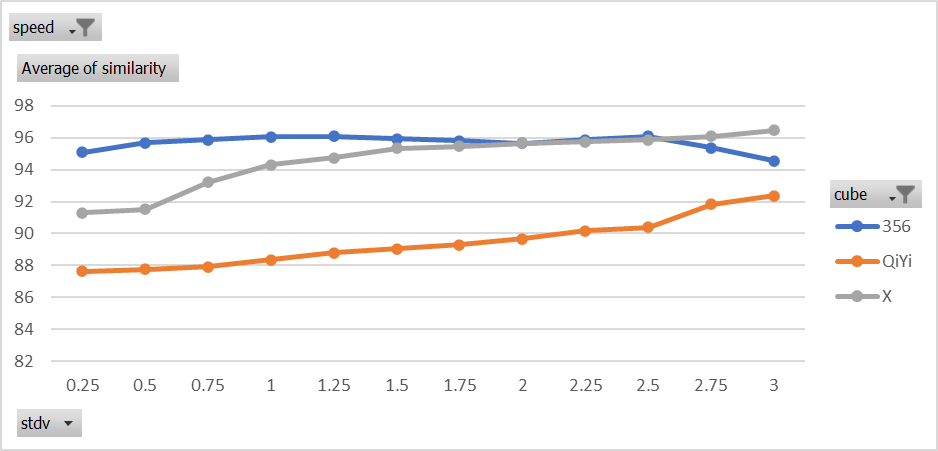
\includegraphics[width=0.75\linewidth]{Figures/7 Evaluation/similarity_by_cube_2tps.png}
\end{figure}

Basically the same as the overall average, just higher numbers overall.

\begin{figure}[h]
    \centering
    \caption{Average across 5 TPS}
    \label{fig:similarity-by-cube-5tps}
    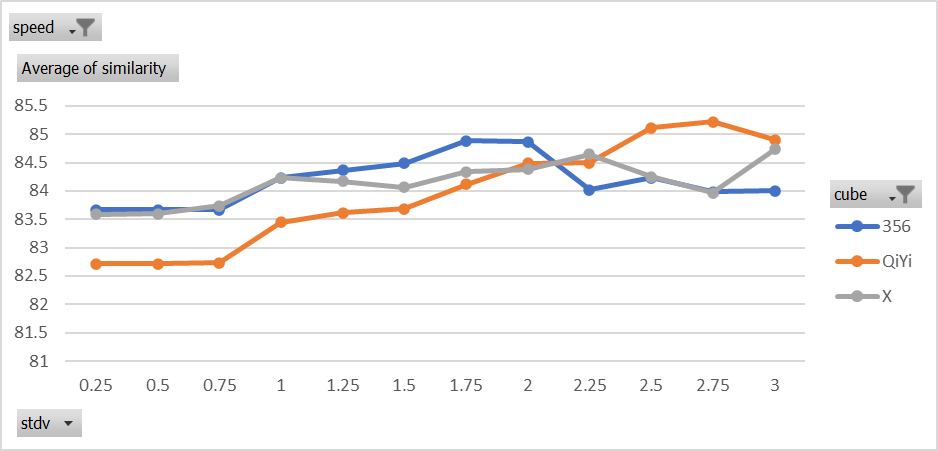
\includegraphics[width=0.75\linewidth]{Figures/7 Evaluation/similarity_by_cube_5tps.png}
\end{figure}

How is this for volatility? 

It's interesting that the 356 and the X start out virtually identical.
Also interesting is that the QiYi achieves the highest overall accuracy
of all three cubes.


\begin{figure}[h]
    \centering
    \caption{Best accuracy for each stdv multiplier}
    \label{fig:max-similarity-by-stdv}
    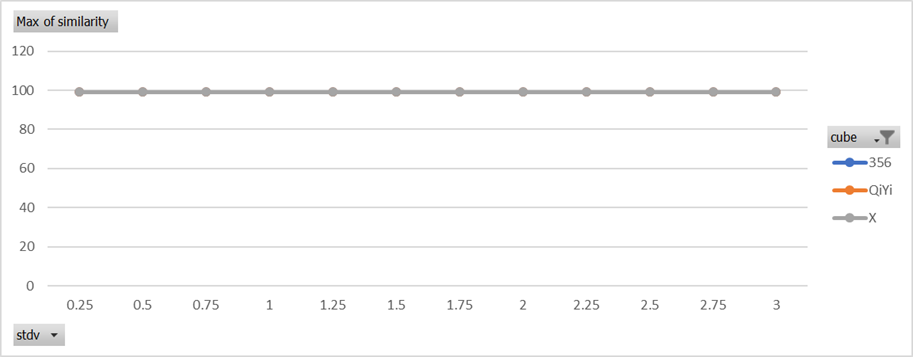
\includegraphics[width=0.75\linewidth]{Figures/7 Evaluation/max_similarity_by_stdv.png}
\end{figure}

\subsection{Influence of Window Size}

\begin{figure}[h]
    \centering
    \caption{Effect of window size on accuracy of detection by cube}
    \label{fig:similarity-by-window-size}
    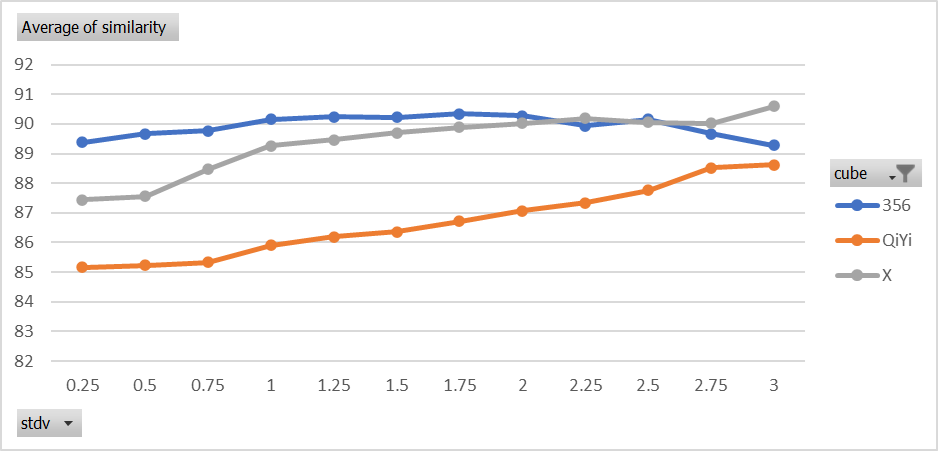
\includegraphics[width=0.75\linewidth]{Figures/7 Evaluation/similarity_by_cube.png}
\end{figure}

A higher window size consistently improved the accuracy of detection.
That said we do start seeing some decreases at a window size of 10, it
would be interesting to see when the window size starts inhibiting
accuracy.

I did not include the breakdown by speed because the graphs are
basically identical.

\begin{figure}[h]
    \centering
    \caption{Best accuracy for each window\_size}
    \label{fig:max-similarity-by-window-size}
    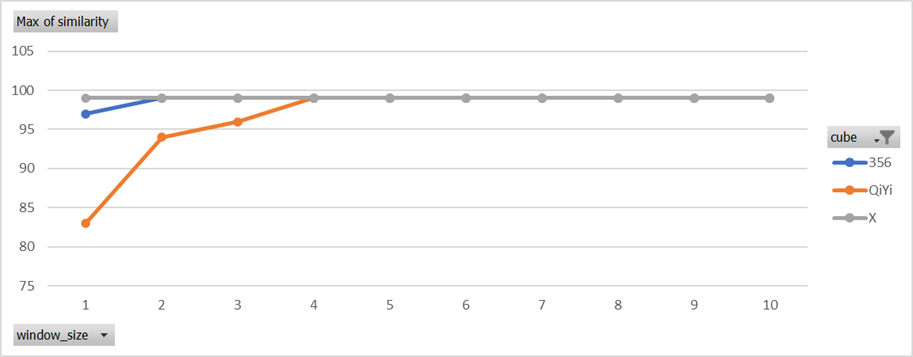
\includegraphics[width=0.75\linewidth]{Figures/7 Evaluation/max_similarity_by_window_size.png}
\end{figure}

\subsection{Influence of Minimum Threshold}

\begin{figure}[h]
    \centering
    \caption{Effect of alt\_min on accuracy of detection by cube}
    \label{fig:similarity-by-alt-min}
    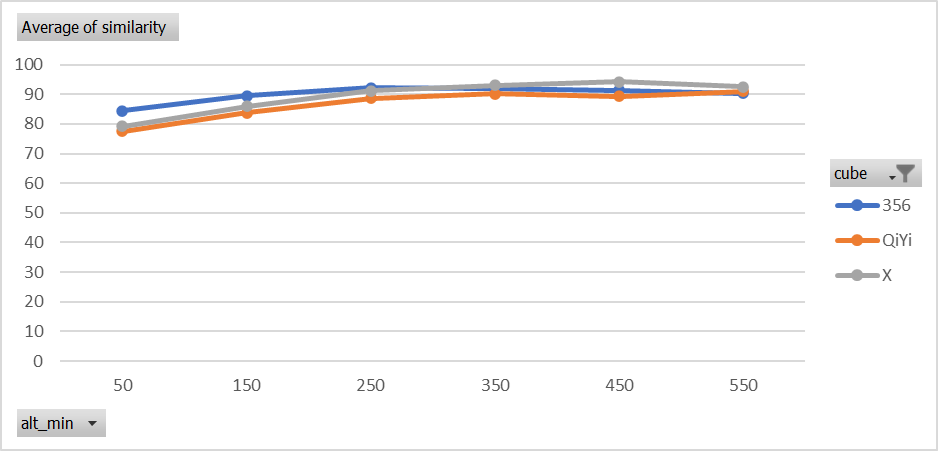
\includegraphics[width=0.75\linewidth]{Figures/7 Evaluation/similarity_by_alt_min.png}
\end{figure}

Like the window\_size, a higher alt\_min tends to correlate with a
higher accuracy; however, a low alt\_min doesn't hurt nearly as much as
a low window\_size.

\begin{figure}[h]
    \centering
    \caption{Best accuracy for each alt\_min}
    \label{fig:max-similarity-by-alt-min}
    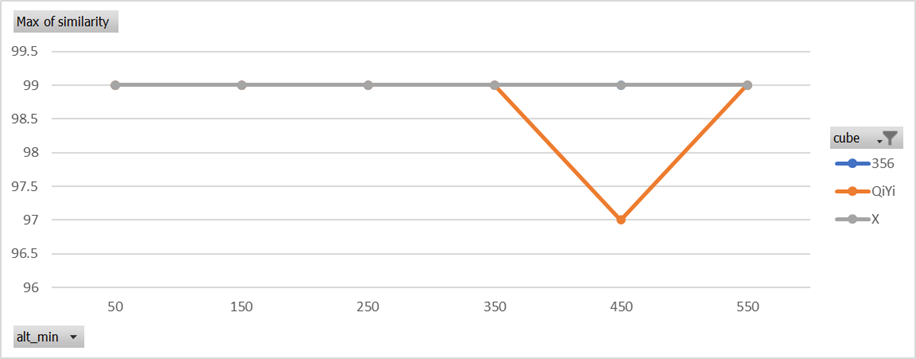
\includegraphics[width=0.75\linewidth]{Figures/7 Evaluation/max_similarity_by_alt_min.png}
\end{figure}


\section{Move Tracking Granularity}
\label{sec:move-tracking-granularity}

While tracking the moves performed on the speedcube constitutes the
minimum viable functionality for a design, additional features make a
design a more useful solution to the speedcubing community. Of most
value is the ability to track the amount of time spent performing each
face turn; from that single metric many other highly valuable metrics
can be derived like TPS over time, and time spent completing each stage
of the solution.

Though not shown in the pretty printed algorithm from Section
\ref{subsec:ignoring-noise-when-extracting-move-sequences}, the
proposed software receiver also records the time stamp at which it
detected each face turn. By computing the difference between time
stamps, one can calculate the amount of time spent performing each
individual face turn. While not implemented in this design, a more
sophisticated software receiver could provide even more precise
measurements from the same source data by measuring the amount of time
between stable signals for each centerpiece state.

However, since this design does not include a gyroscope, it cannot
provide metrics about cube orientation over time like the highest-end
commercial smartcubes. As such, this design cannot be used to directly
report x, y, and z cube rotations, those sophisticated post-processing
heuristics could predict their locations with decent accuracy.


\section{Competition Legality}
\label{sec:competition-legality}

As discussed in Section \ref{subsec:competition-regulations},
speedsolving competitors cannot use any electronics or audio equipment
while solving the cube in competition. Since a major goal of this
research project is to allow speedcubers to practice with the same cube
they compete with, a design must either inherently comply with existing
competition rules against the use of electronics or must result in a
cube that can be easily modified to regain compliance.

While the design proposed in this thesis, certainly does not inherently
comply with the existing competition regulations since it requires
embedding electronics into the cube, it does result in a cube that can
be easily modified to regain compliance. As mentioned in Section
\ref{sec:compatibility-with-standard-speedcubes}, the only modification
to the cube is an interchangeable centercap that can be easily removed
and replaced with the original centercap to produce a perfectly
competition-legal cube.

Interestingly, the sound-based nature of this design provides a
potential compromise on the use of smart cubes in competition. As
mentioned at the end of Section \ref{sec:minimizing-sound-obstruction},
a sound-based transmitter only works at a short range and can easily be
rendered inaccessible to a competitor by scrambling cubes several
meters away from the competitors (especially in a different room), or
playing audio at the same frequencies as the transmitter. As such,
these properties of sound-based turn tracking could provide an avenue
in which smart cubes could be safely allowed in competitions to aid in
solve reconstructions without enabling competitors to spy on scrambles.

\section{Summary}
TODO write the chapter summary

